\chapter{Modelos de Negocio}
\label{CHAP3:Economy}

En este capítulo la idea fundamental que se va a presentar es ¿Quién paga el
desarrollo de los programas?, ¿Por qué alguien paga por un software?, ¿Cómo
financiar proyectos y recursos?
% <+> 
Dejaremos de un lado los aspectos éticos y nos centraremos en los
modelos prácticos que permiten obtener beneficios, no siempre
económicos.
% </+>

La financiación de los proyectos pueden llegar de diferentes maneras:

\begin{itemize}
  \item Financiación externa. Alguien financia el proyecto y decide cómo y en
  qué se gastan los recursos.
  \item Autofinanciados. La financiación proviene de las actividades de la
  empresa.
  \item Desarrollos con financiación indirecta. Participación de desarrolladores
  en proyectos pero que trabajan para otras empresas.
  \item Desarrollo para uso interno.
  \item Modelos mixtos. Una pequeña mezcla de los anteriores.
\end{itemize}

A continuación vamos a comentar más en detalle cada uno de los tipos.


\section{Financiación externa}

Como bien indica el título de esta sección, la financiación proviene de una fuente externa
que por diversos motivos quiere que el software sea libre. En los siguientes
apartados vamos a poder ver las diferentes formas de financiación externa que
existen.

\subsection{Empresa pública}


La empresas públicas tiene diversos modelos de financiación, uno de ellos es
del tipo I+D y se decide que para poder financiar un proyecto, éste tendrá que
ser libre.

Otro modelo de financiación es crear proyectos competitivos, como por ejemplo
con los planes Avanza, que se evalúan según lo que pueden ofrecer a la
investigación. Éstos pueden ser software libre.
% <+> 
También hay cabida para motivación precompetitiva, donde se
pretende desarrollar una tecnología que pueda ser explotada en el
futuro por determinadas empresas. El acceso público al programa
permite que el rango de grupos que pueden hacer uso de él sea mucho
más grande, favoreciendo la entrada de PYMES y modestos proyectos de
investigación.
% </+>

Muchas veces con este tipo de financiación no se busca recuperar la inversión,
aunque hay casos en los que se puede recuperar mediante subproductos, pero no
es la idea.
% <+>
Un ejemplo de esto puede ser el provecho que la sociedad obtiene por
la inversión en tecnologías sanitarias para un hospital público.
% </+>

Las motivaciones para la financiación de este tipo de proyectos son variadas,
como científicas, precompetitivas, promocionales, sociales o políticas.
% <+> 
En las científicas podemos encontrar, por ejemplo, estudios en
biotecnología, donde los resultados pueden ser reutilizados por otras
entidades. En cuanto a las precompetitivas, se busca que todo el tejido
industrial se pueda beneficiar de esos resultados precompetitivos, siendo el
software libre en este caso, tal y como se ha podido comprobar, un claro
vehículo para conseguirlo, ya que al finalizar la producción de ese software,
se libera (téngase en cuenta que se subvenciona el software no sólo para su
producción sino para su posterior liberación) quedando a disposición de
todos, incluso para aquellos que no pertenecen al consorcio del proyecto. Las
promocionales se basan generalmente en extender un estándar, donde el ejemplo
más ilustre es el de Internet. Gracias a los reducidos costes que suponía
implantar TCP, fueron muchos los fabricantes que se lanzaron a incluirlo en sus
productos. En cuanto a la motivación social, se hace presente en ciertas
ocasiones cuando sale más rentable crear un producto desde cero y publicarlo
como Software Libre que financiar otro producto de pago ya existente. Un
ejemplo de esto sería imaginar una sociedad en la que no existiesen
navegadores web gratuítos.
% </+>

Un caso de estudio importante en esta sección es el del compilador de lenguaje
Ada llamado GNAT. Su principal objetivo era conseguir un compilador muy barato,
pero su calidad y éxito fue tal que llegó a expulsar del mercado a otros
compiladores de Ada privativos. La clave de su éxito (y de su coste
reducido) se encontró en que no se realizó un desarrollo del mismo desde cero,
sino que se reutilizaron otros programas de software libre como el compilador
de C, GCC. En definitiva, el esfuerzo se centró en la creación del front-end
para la sintaxis del lenguaje, dado que el resto de componentes ya estaban
hechos.

Dentro de la financiación externa, existen algunas variantes de las cuales
hablaremos a continuación.

\subsection{Empresa privada sin ánimo de lucro}

Normalmente esta financiación está realizada por fundaciones u ONGs, ya bien
sea para producir software o para solucionar problemas mediante el desarrollo de
software.

% <+>
Los motivos de la entidad financiadora suelen ser directos, como el
caso de la FSF cuya meta es la proliferación del software libre, o
indirectos como la fundación Open Bioinformatics, que se vale del
software libre como medio para extender sus productos. También se
pueden encontrar aquí ejemplos de tecnología de geolocalización, para
desplegar las posiciones de víctimas, puestos sanitarios o puntos de
repartición de alimentos tras producirse desastres naturales.
% </+>

La forma de financiar los proyectos es muy parecida a la que se usa en las
empresas públicas.


\subsection{Porque alguien necesita mejoras}
En este caso sí existe el ánimo de lucro. El proyecto en cuestión se financia
porque va a realizar mejoras a un software que necesito.
Esta financiación se puede hacer de varias maneras:
\begin{itemize}
  \item Pagando a una empresa externa.
  \item Pagando a una fundación.
  \item Contratando personal.
\end{itemize}

De cualquiera de las tres maneras se estaría financiando el proyecto del cual
finalmente saldremos beneficiados.


Uno de los casos es \emph{Corel}, empresa que quería portar todo su software a Linux para
poder competir con Microsoft. Y lo que decidieron es usar un emulador llamado
\emph{Wine}, y lo financiaron para que sus aplicaciones funcionaran bien en
Linux, y pagaron a una empresa llamada \emph{Macadamian} para que lo realizase.

\subsection{Indirecta}

La idea de la financiación indirecta es que financio un proyecto, no tanto
porque me interese el proyecto en sí, sino por los productos que puedan salir de
él. En el caso de Google, por ejemplo, que financia un proyecto de software
libre y obtiene un producto como Android.

Google se introduce en el mercado móvil para poder tener control y estar de
intermediarios de todo lo posible como publicidad, aplicaciones, etc\ldots
Crean un sistema operativo como Android, no para ganar dinero con Android, pero
si para no dejar que otros le quiten el poder de ser intermediarios y ser competitivos.
Buscan beneficios en productos relacionados con Android, no del propio Android.
Y el software libre es el instrumento para hacerlo. Intentar obtener céntimos
por cada compra/venta en el mundo con sus productos. La ganancia de Android, es
que lo pueda usar mucha gente y cuanta más gente mejor, bien en dinero o bien en
control.

En el caso de VISA/MASTERCARD hacen algo de este estilo, y la idea de Apple o
Google es ésta. RIM está creando WebOS con software libre pero es privativo.

Tenemos varios ejemplos:
\begin{itemize}
  % <->
  %\item Con Perl, crearon el software y se recuperó el dinero vendiendo libros.
  %Cuantos más usuarios de Perl más gente compraría el libro. Y en vez de
  %pagar por crear el libro, se pagó porque Perl fuese mejor y tuviese más
  %versiones.
  % </->
  % <+>
  \item En ocasiones, una entidad invierte en cierta tecnología con el
    fin de obtener más ventas en productos relacionados donde tienen
    una alta cuota de mercado. Esta estrategia ha sido realizada en
    varias ocasiones por la editorial O'Reilly. El caso más conocido
    es el de su guía sobre el lenguaje de programación Perl. Su libro
    se convirtió en el mayor referente sobre el tema. Por ello
    a la editorial le resultaba rentable invertir capital en el
    desarrollo de este lenguaje. Bien es cierto que terceras partes
    también se lucraban sin gasto alguno con las inversiones
    realizadas por O'Reilly, pero era un factor que no les preocupaba,
    siempre y cuando no cesase su propio crecimiento.
  % </+>
  \item Con el Hardware, VA (VA-Linux) vendía servidores, y lo que hace ahora es vender
servidores con Linux preinstalado y pagó para que las versiones de Linux
de sus servidores corriesen muy bien y sin problemas. 
% <+>
Es cierto que no existía mucho mercado para máquinas con Linux
preinstalado, pero tener una cuota del 80\% de dichas ventas suponía
unos ingresos elevados.
% </+>
Hay casos en los que se
pagan para que hagan el driver para ciertas tarjetas y cuando están disponibles
para Linux su venta aumenta.
\item Otro caso son las distribuciones de Linux, como Ubuntu, que paga para
que la distribución sea conocida y mucha gente la utilice.
% <+>
Ubuntu invierte una gran cantidad en lograr una buena usabilidad y
mejorar la experiencia de usuario. Otras distribuciones como Red Hat
utilizan las certificaciones y consultorías como principal fuente de
ingresos. En ambos casos, lograr que el nombre de la empresa sea
conocido es de vital importancia.
% </+>
\end{itemize}

% <+>
\subsection{Otros modos}
Obtener los ingresos mediante otros mecanismos ajenos a la venta de
licencias, tal y como ocurría en el modelo tradicional, ha llevado a
modelos muy dispares e imaginativos de financiación. Por citar alguno,
podríamos hablar de mercados puntos de encuentro entre desarrolladores
y clientes, venta de bonos para financiación (utilizado por el
proyecto Diaspora), cooperativas de desarrolladores y sistemas de
donaciones (de manera directa realizando una transferencia o con
cierta indirección, como la existente en el market de Android, donde
puedes elegir obtener la misma aplicación sin coste alguno o
pagando un precio razonable a modo de donación).
% </+>

\section{Autofinanciados}

Con la autofinanciación soy yo el que invierte en el desarrollo y luego
trato de recuperarlo de alguna manera.

Estos casos se darían cuando por ejemplo, una empresa quisiera iniciar un
proyecto libre destinado a un determinado nicho de mercado en el que ve
posibilidades de negocio futuro y por tanto, con la idea de rentabilizar a
posteriori esa inversión inicial.

Como se puede entender, mediante este tipo de financiación se pueden originar
diversos modelos de negocio que veremos en este apartado.

\subsection{Mejor conocimiento}

La idea es tratar de vender que tengo el mejor conocimiento de un producto, esto
puede hacer que después cuando haya que realizar un cambio pueda ofrecer precios
más baratos que si lo hace otro porque conozco muy bien el producto o bien para
intentar obtener una marca. Esto se puede dar o bien desarrollando el propio
programa o bien trabajando en otro software que ya existe.
% <+>
La manera más habitual de vender un buen conocimiento es mediante la
inclusión de varios desarrolladores oficiales del proyecto en el
propio equipo de trabajo.
% </+>

Si tenemos un buen conocimiento de un producto podemos vender consultoría,
adaptación, integración, etc\ldots

Intentar que alguien use mucho el software y luego me paguen por hacer
modificaciones o añadir servicios.

Algunos casos, pueden ser:
\begin{itemize}
  \item Levanta, dan consultoría y soporte GNU/Linux y software libre en EEUU.
  \item Alcove, daba consultoría y consultoría estratégica para software libre
  en Europa.
\end{itemize}

% <+>
Generalmente, para implantar este modelo, se suele hacer una inversión
inicial muy fuerte y se espera que el dinero vaya llegando con el
tiempo. Por ser una práctica con cierto riesgo, se suelen realizar
estudios de mercado previos.
% </+>

\subsection{Mejor conocimiento con limitaciones}

El tener el mejor conocimiento tiene la limitación de que el resto también
puedan conseguirlo. Aunque existe otra forma que se llama tener
mejor conocimiento con limitaciones.

Este modelo intenta limitar el problema que teníamos anteriormente de que la
competencia también sea experta en el mismo producto que tú. Para ello se
utilizan licencias, en las que tienen una parte privativa y una parte libre. De
manera que la parte privativa esta más enfocada para dar servicio a empresas y
éstas tienen que pagar y una parte libre más enfocada para todo el mundo.
Normalmente la parte privada tendrá componentes o servicios que no tendrá la
libre, y así potencias que paguen la licencia.

El problema que tiene esto es que las comunidades, pueden crear las partes
que falten en la parte privativa y eso te hará perder marca y ser el productor
principal. Como es el caso de OpenOffice y LibreOffice.

% <+> 
Otro contexto en el que se utiliza este modelo es cuando una empresa o
individuo es poseedor de cierta patente, lo que imposibilita
legalmente que determinada parte pueda ser reimplementada por terceras
personas.
% </+>

Los proveedores de CRM hacen cosas de este estilo.


\subsection{Fuente de un programa}

Ser la fuente de un programa. Es la idea de tener una marca y ser el punto de
referencia sobre un producto. Es más terminos de imagen, como Sun con OpenOffice.

Otro ejemplo claro es IBM que financia Eclipse y esto da una sensación de que
IBM hace cosas serias. Presumiblemente, este sería el mismo caso de Sun
Microsystems con OpenOffice, es decir, la búsqueda de una buena imagen de
marca, y más teniendo en cuenta que no está del todo claro que Sun llegase
nunca a tener ingresos directos en concepto de OpenOffice. Además, se debe
tener en cuenta que apadrinar un producto como Eclipse en el caso de IBM, a
veces puede resultar menos costoso que el hecho de obtener publicidad mediante
vías más tradicionales.

Finalmente la financiación se termina rentabilizando en términos de imagen de
marca.

Algunos ejemplos más de esto son:
\begin{itemize}
 \item Abiword, intentó crear una suite ofimática, pero cuando OpenOffice se liberó,
pues no consiguieron seguir.
\item Evolution, RedCarpet, creada por Ximian, las regalaban en las
aplicaciones, finalmente se vendieron a Novel, para recuperar el dinero
invertido para crear Evolution. Mucha gente les conocía y estaban en una buena
posición dentro del mercado.
\item Zope, tenía un producto privativo, cuando fueron a pedir financiación, la
empresa les dijo que sólo les financiaba si lo hacían libre, de esta manera se
ha creado una gran comunidad alrededor de Zope.
\item Por último, el caso de Asterisk, que se espera que sea el centro para la
gestión de centralitas para su uso en VoIP.
\end{itemize}



\subsection{Fuente de un programa con limitaciones}

Otra forma de poner limitaciones a la competencia es que primero puedo hacer el
producto privativo y cuando me interese lo libero, de esta manera la competencia
irá retrasada con respecto a mí.

Un caso claro es lo que está haciendo Google con la última versión de Android,
primero se la facilita a los fabricantes de móviles para que puedan adaptarlas a
su manera, y cuando éstos ya están disponibles en el mercado, libera la versión
para el resto del mundo.

Aunque hay que decir que esto no siempre funciona.

\subsection{Licencias especiales}
Es una variante del apartado anterior, lo único es que lo hago a la vez.
Pero la versión privativa me permite crear trabajos
derivados de ella y puedo ponerle la licencia que yo quiera. En cambio, la
versión libre siempre llevará una licencia GPL y si alguien realiza una versión
derivada, tendrá que añadir esta licencia.

Según el modelo de negocio dependerá mucho de las licencias que uses.

\subsection{Venta de marca}
Lo único que quiero es vender marca, del estilo de Red-Hat. Vende servicios
alrededor de su marca, sólo por tener la marca la gente ya va a pagar porque
tienes una imagen detrás que respalda el trabajo que realizas.

\section{Desarrollos sin financiación directa}
Es posible que existan proyectos en los que haya desarrolladores que sus
propias empresas les dejan trabajar para otros proyectos de software libre, bien
en su tiempo libre o bien ciertas horas al día.

Aunque no están financiados sí reciben alguna contribución, como parches por
alguna cierta funcionalidad, donación de máquinas como infraestructura,
donaciones propias, etc\ldots


\section{Desarrollos para uso internos}
Este tipo de financiación está basada en que yo necesito algo y lo desarrollo como
software libre, de esta manera al publicarse, el código estará más limpio y en un
futuro puedo encontrar colaboración.

% <+>
Un ejemplo de este modelo es el que utilizó Cisco en un sistema de
gestión de impresoras. Llegaron a la conclusión de que no perderían
nada con su liberación y que era una manera de mejorarlo. Otro efecto
colateral era sobre el ánimo de los desarrolladores, ya que estaban
más motivados por trabajar en un proyecto con visibilidad externa.
% </+>


\section{Clasificación de Hecker}

A lo largo de este capítulo se ha estudiado una posible clasificación para los
diversos modelos de negocio entorno al \textit{software} libre. Pero por
supuesto, existen múltiples clasificaciones, entre las cuales destaca la
realizada por Hecker y que fue adoptada por la \textit{Open Source Initiative}.
Quizás la peculiaridad de esta clasificación reside en que para determinados
modelos, el \textit{software} no ocupa un lugar de verdadera relevancia sino que
más bien supone un acompañante que ofrece valor añadido al producto
final\footnote{Tabla extraída del libro ``\textit{Handbook of Research on Open
Source Software: Technological, Economic, and Social Perspectives}'', de Kirk
St. Amant y Brian Still}. Pese a todo, se pueden encontrar correspondencias
directas entre algunos de los modelos de la clasificación de Hecker y
algunos otros de los estudiados con detenimiento a lo largo del capítulo.

\begin{figure}[htb]
  \centerline{\resizebox{\textwidth}{!}{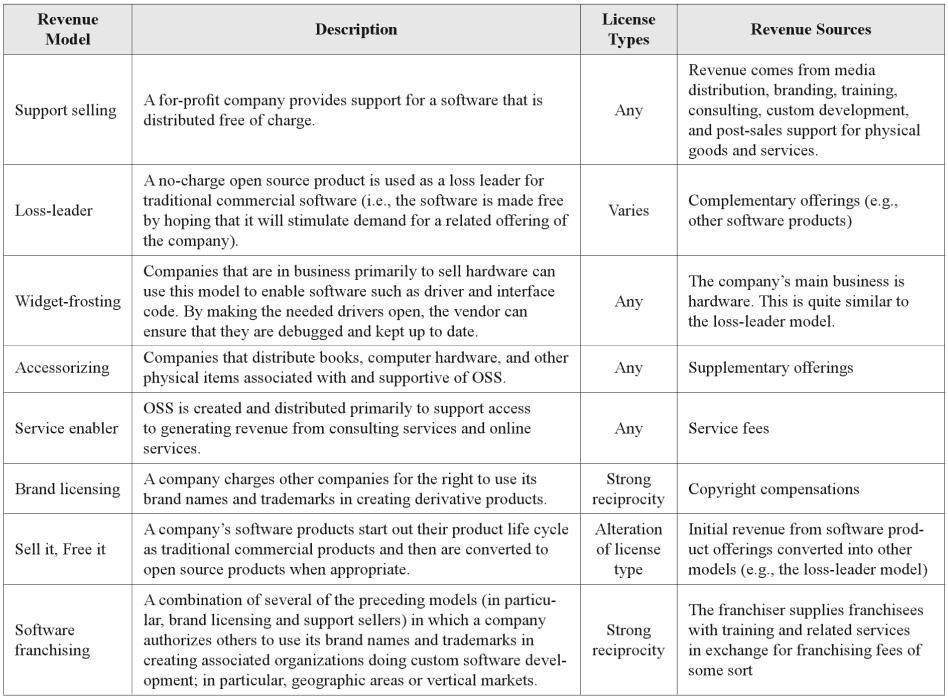
\includegraphics{img/hecker}}}
  \label{IMG:Hecker}
\end{figure}

\section{Otros modos de financiación}

Existen otros modos de financiación cuya cabida dentro de alguna de las
categorías estudiadas en las clasificaciones anteriores resulta complicada.
Algunas de ellas pueden ser:

\begin{itemize}
  \item Mediante sitios en los que se ponen en contacto desarrolladores y
clientes, de tal modo que un desarrollador indica su perfil y habilidades,
mientras que los clientes publican sus necesidades, de tal modo que puedan
llegar a un acuerdo contractual para el producto. Un claro ejemplo de este
modelo se ejemplifica a través de SourceXchange.
  \item Mediante venta de bonos que cotizasen al estilo de una bolsa o mercado
de bonos. El funcionamiento simplificado de una de sus variantes más extendidas
sería el siguiente: un desarrollador tiene una idea para un nuevo programa o
mejora de otro ya existente, ante lo cual, indica sus requisitos,
especificación, presupuesto, etc. Se generan unos bonos y en caso de que el
presupuesto indicado haya sido cubierto (el desarrollador ha vendido los bonos
suficientes como para ello), el desarrollador comienza a trabajar en ese
software, teniendo siempre en cuenta que si el proyecto no llega a ejecutarse,
la donación en forma de esos bonos es devuelta a sus depositarios. De esta
manera comenzó el trabajo en la red social distribuida Diaspora, mediante este
modelo que ha dado en llamarse financiación de las masas (Cloud Sourcing) y que
es un ejemplo más de las nuevas formas de colaboración que permite la
tecnología.
  \item Mediante cooperativas de desarrolladores, de modo que los
desarrolladores de software libre, en lugar de trabajar individualmente, se
reúnen a través de algún tipo de asociación similar a una cooperativa y con un
funcionamiento parecido al de una empresa, salvando el carácter ético con el
mundo del software libre. Un ejemplo de este tipo de organizaciones es Free
Developers.
  \item Mediante un sistema de donaciones (similar a la venta de bonos) en el
que los usuarios interesados en que un proyecto continúe lanzando nuevas
versiones, pueden realizar un pago/donación a su autor de manera voluntaria a
través de su página web y sirviendo como método de financiación para dicho
desarrollador.
\end{itemize}

\section{Modelos Mixtos}

A modo de resumen, cabe resaltar que en la práctica, las empresas llevan a cabo
estrategias basadas en la combinación de varios de los modelos de negocio aquí
vistos, dándose origen por lo tanto a modelos mixtos. Es más, tanto es así, que
en raras excepciones esas empresas se dedican únicamente al software libre
(quizás el más claro de los ejemplos sea el caso de Google, que si bien
capitanea la plataforma Android, no libera el código fuente y algoritmos de su
buscador y demás servicios en línea). En cualquier caso, es muy destacable
analizar cómo cada vez más empresas consideradas como ``tradicionales'' en el
mundo de la computación, cada vez con más frecuencia prueban líneas de negocio
basadas en el software libre o lanzan proyectos de este tipo como producto
estratégico en un determinado mercado, así como el hecho mismo de intentar
fortalecer la imagen de marca.

